\section{Ứng dụng Deep Learning cho bài toán Multi-class / Multi-label}

Các phần trước đã trình bày cơ sở lý thuyết và các thuật toán nền tảng cho phân loại đa lớp/đa nhãn, gồm Multi-class SVM, AdaBoost.MH, Decision Tree, One-vs-All, One-vs-One, ECOC và dự đoán có cấu trúc. Các phương pháp này có ưu điểm là rõ ràng về mặt mô hình hóa và dễ phân tích. Tuy nhiên, khi dữ liệu đầu vào là văn bản dài, ảnh, âm thanh hoặc dữ liệu y sinh, việc thiết kế đặc trưng thủ công như TF-IDF hay vector thống kê đơn giản thường không đủ để biểu diễn ngữ nghĩa sâu của dữ liệu.

Deep Learning được xem như một hướng mở rộng tự nhiên vì mô hình có thể học biểu diễn trực tiếp từ dữ liệu đầu vào, đồng thời học chung nhiều đầu ra trong cùng một kiến trúc. Với bài toán multi-label, điều này đặc biệt quan trọng vì các nhãn thường không độc lập hoàn toàn: một ảnh có thể đồng thời chứa người, xe và đường phố; một văn bản có thể vừa thuộc chủ đề thể thao vừa thuộc chủ đề sức khỏe. Vì vậy, trọng tâm của phần này là chỉ ra cách mạng nơ-ron được điều chỉnh để xử lý đầu ra đa lớp/đa nhãn.

\begin{figure}[htbp]
    \centering
    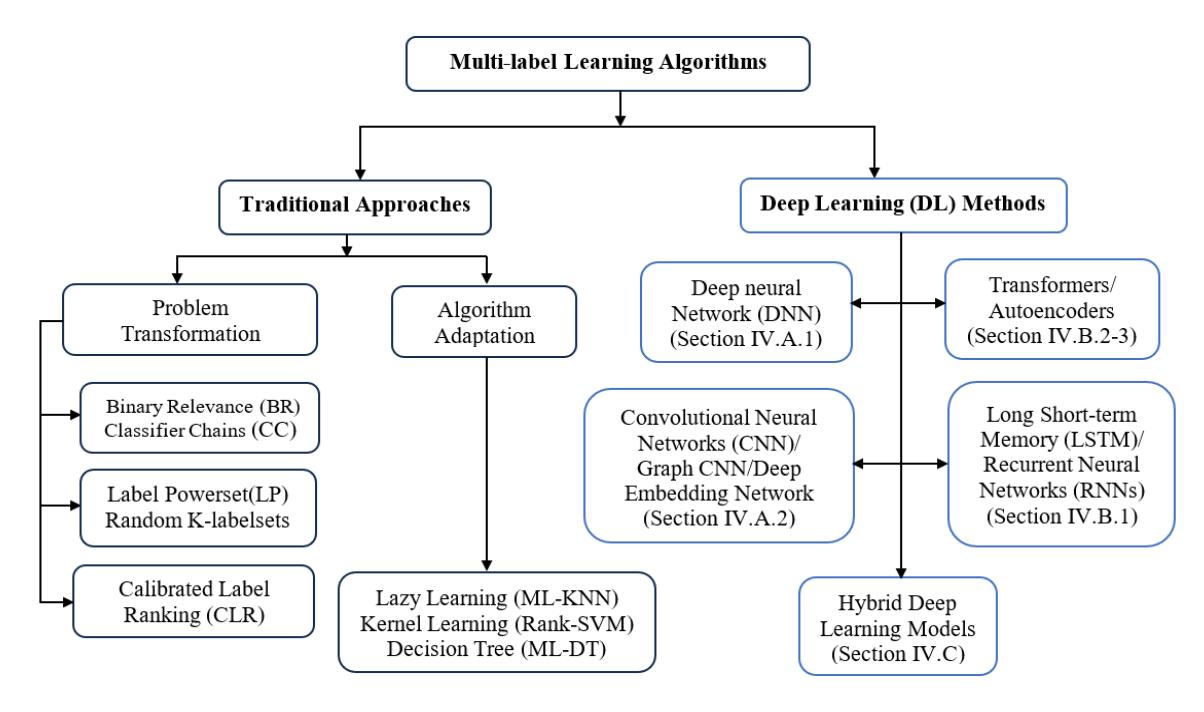
\includegraphics[width=0.88\textwidth]{figures/dl_mlc_taxonomy.jpeg}
    \caption{Phân loại tổng quát các hướng tiếp cận trong multi-label learning: nhóm truyền thống và nhóm Deep Learning.}
    \label{fig:dl_mlc_taxonomy}
\end{figure}

\subsection{Đầu ra và hàm mất mát trong mạng nơ-ron}

Ở các phần trước, bài toán phân loại đa lớp đã được mô tả thông qua hàm điểm số
$h(x,y)$ và quy tắc chọn nhãn có điểm số lớn nhất. Trong mạng nơ-ron, tầng cuối
thường sinh ra một vector điểm số chưa chuẩn hóa, gọi là \textit{logits}. Cách chuyển
logits thành dự đoán phụ thuộc vào việc bài toán là đơn nhãn hay đa nhãn.

Với bài toán multi-class đơn nhãn, mỗi mẫu chỉ thuộc đúng một lớp trong
$\{1,2,\ldots,k\}$. Vì các lớp loại trừ nhau, tầng đầu ra thường dùng softmax:
\[
    p(y=l\mid x)
    =
    \frac{\exp(z_l)}
    {\sum_{j=1}^{k}\exp(z_j)},
    \qquad l=1,\ldots,k.
\]
Khi đó, các xác suất trên $k$ lớp có tổng bằng $1$ và mô hình dự đoán lớp có xác
suất lớn nhất:
\[
    \hat{y}=\arg\max_{l} p(y=l\mid x).
\]
Hàm mất mát thường dùng là cross-entropy đa lớp:
\[
    \mathcal{L}_{CE}
    =
    -\frac{1}{m}
    \sum_{i=1}^{m}
    \log p(y_i\mid x_i).
\]

Với bài toán multi-label, một mẫu có thể đồng thời mang nhiều nhãn. Do đó, các nhãn
không được chuẩn hóa cạnh tranh như softmax. Nếu có $L$ nhãn, tầng đầu ra thường
gồm $L$ nút sigmoid:
\[
    p_{il}
    =
    \sigma(z_{il})
    =
    \frac{1}{1+\exp(-z_{il})},
    \qquad l=1,\ldots,L.
\]
Mỗi $p_{il}$ biểu diễn xác suất mẫu $x_i$ mang nhãn $l$. Nhãn dự đoán thường được
xác định bằng một ngưỡng $\tau_l$:
\[
    \hat{y}_{il}
    =
    \begin{cases}
    1, & p_{il}\geq \tau_l,\\
    0, & p_{il}<\tau_l.
    \end{cases}
\]
Hàm mất mát phổ biến là binary cross-entropy theo từng nhãn:
\[
    \mathcal{L}_{BCE}
    =
    -\frac{1}{m}
    \sum_{i=1}^{m}
    \sum_{l=1}^{L}
    \left[
    y_{il}\log(p_{il})
    +
    (1-y_{il})\log(1-p_{il})
    \right].
\]

Lưu ý rằng đầu ra sigmoid chỉ xem mỗi nhãn như một quyết định nhị phân ở tầng
cuối. Điều này không có nghĩa toàn bộ mô hình học các nhãn hoàn toàn tách rời. Trong
mạng nơ-ron, các tầng ẩn phía trước vẫn được học chung, nên mô hình có thể chia sẻ
biểu diễn giữa những nhãn có liên quan. Nếu muốn khai thác quan hệ nhãn rõ hơn,
các kiến trúc như attention, RNN/LSTM, Transformer hoặc graph thường được đặt ở
phần encoder trước khi đưa ra dự đoán cuối cùng.

\begin{table}[htbp]
\centering
\small
\renewcommand{\arraystretch}{1.25}
\begin{tabular}{p{0.23\textwidth} p{0.34\textwidth} p{0.33\textwidth}}
\hline
\textbf{Thiết lập}
& \textbf{Tầng đầu ra và loss}
& \textbf{Ý nghĩa dự đoán} \\
\hline

Multi-class đơn nhãn
&
Softmax trên $k$ lớp, thường dùng cross-entropy đa lớp.
&
Các lớp loại trừ nhau. Mỗi mẫu được gán đúng một nhãn bằng quy tắc
$\hat{y}=\arg\max_l p_l$. \\

\hline

Multi-label cơ bản
&
Sigmoid riêng cho từng nhãn, thường dùng binary cross-entropy theo từng nhãn.
&
Mỗi nhãn là một quyết định nhị phân. Một mẫu có thể đồng thời nhận nhiều nhãn
nếu $p_l \geq \tau_l$. \\

\hline

Multi-label có mô hình hóa quan hệ nhãn
&
Dùng encoder chung, attention, RNN/LSTM, Transformer hoặc graph trước tầng
sigmoid/ranking.
&
Mô hình không chỉ học đặc trưng đầu vào mà còn khai thác quan hệ đồng xuất hiện,
thứ tự hoặc cấu trúc giữa các nhãn. \\

\hline
\end{tabular}
\caption{So sánh tầng đầu ra của mạng nơ-ron trong bài toán multi-class và multi-label.}
\label{tab:dl_output_layer}
\end{table}

\subsection{Các kiến trúc học sâu tiêu biểu}

\paragraph{Mạng truyền thẳng và BP-MLL.}
Cách mở rộng đơn giản nhất là dùng một mạng nhiều tầng với $q$ nút đầu ra, mỗi nút tương ứng với một nhãn. Mô hình BP-MLL là một trong những hướng đầu tiên áp dụng mạng nơ-ron cho multi-label classification. Thay vì chỉ đo sai số từng nhãn riêng lẻ, BP-MLL tối ưu sao cho điểm của các nhãn đúng cao hơn điểm của các nhãn sai. Cách làm này phù hợp để minh họa bước chuyển từ các bộ phân loại nhị phân độc lập sang một mô hình học chung nhiều đầu ra.

\begin{figure}[htbp]
    \centering
    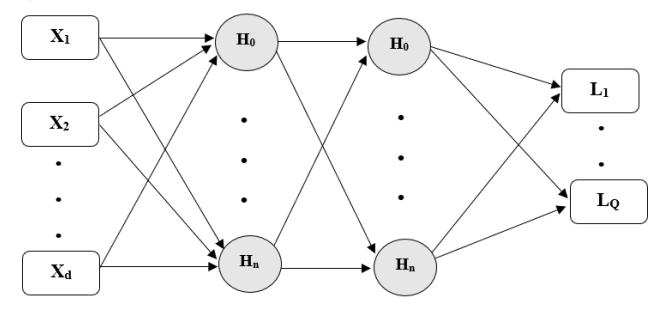
\includegraphics[width=0.68\textwidth]{figures/dl_mlc_dnn.jpeg}
    \caption{Mạng nơ-ron truyền thẳng cho multi-label classification: các đặc trưng đầu vào được ánh xạ qua tầng ẩn đến nhiều nút đầu ra, mỗi nút tương ứng với một nhãn.}
    \label{fig:dl_mlc_dnn}
\end{figure}

\paragraph{CNN và Graph CNN.}
CNN phù hợp với dữ liệu có cấu trúc cục bộ như ảnh, văn bản ngắn hoặc tín hiệu. Trong ảnh đa nhãn, một ảnh có thể chứa nhiều đối tượng cùng lúc, nên CNN thường được dùng làm bộ trích xuất đặc trưng, sau đó tầng đầu ra sigmoid dự đoán xác suất cho từng nhãn. Một số mô hình mở rộng dùng Graph CNN, trong đó mỗi nhãn được xem như một nút trong đồ thị; cạnh giữa các nút biểu diễn quan hệ đồng xuất hiện hoặc quan hệ ngữ nghĩa giữa các nhãn. Cách này giúp mô hình hóa tốt hơn các phụ thuộc nhãn mà CNN thông thường chưa xử lý trực tiếp.

\begin{figure}[htbp]
    \centering
    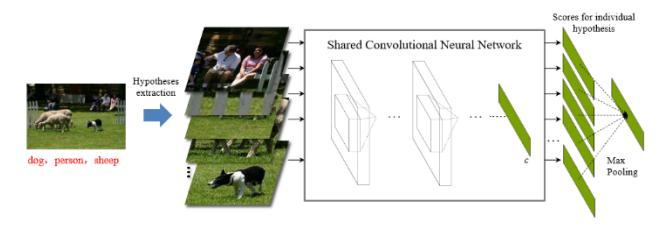
\includegraphics[width=0.82\textwidth]{figures/dl_mlc_cnn_hcp.jpeg}
    \caption{Minh họa hướng dùng CNN cho phân loại ảnh đa nhãn: các vùng/giả thuyết đối tượng được đưa qua CNN dùng chung, sau đó tổng hợp điểm để dự đoán nhiều nhãn.}
    \label{fig:dl_mlc_cnn_hcp}
\end{figure}

\paragraph{RNN/LSTM, Transformer và mô hình lai.}
RNN và LSTM phù hợp với dữ liệu tuần tự như văn bản, chuỗi thời gian hoặc tín hiệu y sinh. Trong multi-label classification, LSTM có thể được dùng để sinh chuỗi nhãn, trong đó nhãn dự đoán trước ảnh hưởng đến nhãn dự đoán sau. Ý tưởng này gần với Classifier Chains, nhưng thay vì dùng nhiều bộ phân loại rời rạc, mô hình học phụ thuộc nhãn trong một kiến trúc tuần tự duy nhất.

\[
    p(y \mid x) = \prod_{t=1}^{n}p(y_t \mid y_1, y_2,\ldots,y_{t-1},x).
\]

Transformer mở rộng hướng này bằng cơ chế attention, cho phép mô hình tập trung vào những phần khác nhau của đầu vào khi dự đoán từng nhãn. Trong xử lý văn bản, các mô hình dựa trên BERT thường cho biểu diễn ngữ cảnh tốt hơn CNN/RNN truyền thống. Trong thị giác máy tính, Transformer hoặc các mô hình lai CNN--Transformer có thể học đồng thời quan hệ không gian giữa vùng ảnh và quan hệ ngữ nghĩa giữa nhãn.

\begin{figure}[htbp]
    \centering
    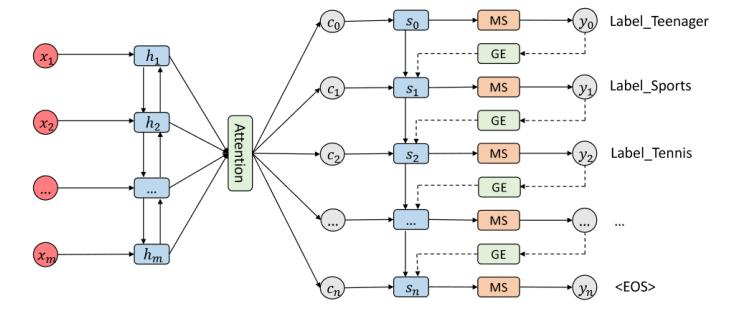
\includegraphics[width=0.82\textwidth]{figures/dl_mlc_lstm_seq.jpeg}
    \caption{Mô hình sinh chuỗi nhãn dùng RNN/LSTM: nhãn ở bước sau được dự đoán dựa trên đầu vào và các nhãn đã sinh trước đó.}
    \label{fig:dl_mlc_lstm_seq}
\end{figure}

\subsection{Liên hệ với các phương pháp truyền thống}

Deep Learning không thay thế hoàn toàn SVM, Decision Tree, OVA hay ECOC trong mọi trường hợp. Khi dữ liệu nhỏ, đặc trưng rõ ràng và yêu cầu diễn giải cao, các mô hình truyền thống vẫn phù hợp. Tuy nhiên, trong những bài toán có dữ liệu phi cấu trúc, quan hệ nhãn phức tạp hoặc số nhãn lớn, mạng nơ-ron thường linh hoạt hơn vì vừa học đặc trưng đầu vào, vừa học biểu diễn dùng chung cho nhiều nhãn.

\begin{table}[H]
\centering
\small
\renewcommand{\arraystretch}{1.25}
\begin{tabular}{p{0.22\textwidth} p{0.34\textwidth} p{0.34\textwidth}}
\hline
\textbf{Hướng tiếp cận} & \textbf{Vai trò } & \textbf{Giới hạn} \\
\hline
SVM, OVA & Nền tảng tuyến tính/kernel, dễ phân tích bằng lề và độ phức tạp. & Khó học quan hệ nhãn nếu các bộ phân loại được học độc lập. \\
Decision Tree & Dễ diễn giải, dự đoán nhanh. & Dễ overfit và không ổn định khi dữ liệu thay đổi. \\
AdaBoost.MH & Xử lý trực tiếp các cặp mẫu--nhãn trong thiết lập đa nhãn. & Chi phí tăng theo số mẫu nhân với số nhãn. \\
DNN/ CNN/ LSTM/ Transformer & Học biểu diễn đầu vào và biểu diễn nhãn trong cùng một mô hình. & Cần nhiều dữ liệu, tốn tài nguyên và khó giải thích hơn. \\
\hline
\end{tabular}
\caption{Liên hệ giữa các phương pháp truyền thống và học sâu trong phân loại đa lớp/đa nhãn.}
\label{tab:traditional_vs_dl}
\end{table}

\subsection{Nhận xét tổng quan}

Vai trò của Deep Learning trong bài toán multi-class/multi-label thể hiện ở hai khía cạnh chính. Thứ nhất, mạng nơ-ron có khả năng tự học biểu diễn đặc trưng từ dữ liệu, thay vì phụ thuộc nhiều vào đặc trưng thủ công như các phương pháp truyền thống. Thứ hai, trong bài toán đa nhãn, các tầng ẩn dùng chung cho phép mô hình chia sẻ thông tin giữa các nhãn; khi kết hợp thêm attention, RNN/LSTM, Transformer hoặc đồ thị nhãn, mô hình có thể khai thác tốt hơn quan hệ đồng xuất hiện, thứ tự hoặc cấu trúc giữa các nhãn.

Tuy nhiên, học sâu không loại bỏ hoàn toàn các khó khăn của bài toán. Các mô hình này thường cần nhiều dữ liệu huấn luyện, chi phí tính toán cao, khó diễn giải hơn so với cây quyết định hoặc mô hình tuyến tính, và vẫn gặp trở ngại khi số lượng nhãn tăng lên quy mô rất lớn. Vì vậy, trong các bài toán extreme multi-label, Deep Learning thường cần được kết hợp với các kỹ thuật giảm không gian nhãn, tạo shortlist hoặc tổ chức nhãn theo cây để đảm bảo khả năng mở rộng.

\section{Các nghiên cứu tiên tiến trong phân loại đa lớp cực đại}

\subsection{Tổng quan Extreme Multi-label Classification}

Trong thực tế, khi số lượng nhãn tăng lên quy mô hàng trăm nghìn hoặc hàng triệu, các thuật toán nền tảng như Multi-class SVM, One-versus-All (OVA) hoặc One-versus-One (OVO) gặp giới hạn nghiêm trọng về chi phí tính toán. Nếu số nhãn là $L$, việc đánh giá trực tiếp hàm điểm cho toàn bộ nhãn thường có độ phức tạp $O(L)$ cho mỗi mẫu, chưa kể chi phí huấn luyện và lưu trữ mô hình.

Extreme Multi-label Classification (XMC) được nghiên cứu nhằm giải quyết tình huống này. Trong XMC, mỗi mẫu có thể gắn với nhiều nhãn, nhưng số nhãn đúng thường rất nhỏ so với tổng số nhãn. Vì vậy, ma trận nhãn có dạng rất thưa và phân phối nhãn thường có tính đuôi dài: một số ít nhãn xuất hiện thường xuyên, trong khi phần lớn nhãn chỉ xuất hiện ở số lượng mẫu hạn chế.

Các thách thức chính của XMC gồm:
\begin{itemize}[leftmargin=2em]
  \item \textbf{Chi phí tính toán:} đánh giá toàn bộ $L$ nhãn là không khả thi khi $L$ rất lớn.
  \item \textbf{Nhãn đuôi:} các nhãn hiếm khó học vì có ít ví dụ huấn luyện.
  \item \textbf{Mất cân bằng dữ liệu:} mô hình dễ thiên về các nhãn phổ biến nếu chỉ tối ưu loss thông thường.
  \item \textbf{Biểu diễn ngữ nghĩa:} Bag-of-Words hoặc TF-IDF có thể không đủ để nắm bắt ngữ cảnh sâu của văn bản.
  \item \textbf{Triển khai thực tế:} hệ thống cần dự đoán nhanh, cập nhật nhãn mới và xử lý văn bản dài.
\end{itemize}

Phần này phân tích một số hướng nghiên cứu tiên tiến giai đoạn 2019--2024, tập trung vào cách các phương pháp hiện đại kế thừa, mở rộng và khắc phục giới hạn của lý thuyết nền tảng về phân loại đa lớp.
\begin{figure}[H]
\centering
\resizebox{0.98\textwidth}{!}{\begin{tikzpicture}[>=Stealth, font=\small]
  \node[align=center, font=\bfseries] at (4.6,4.85) {Phân phối đuôi dài của nhãn};
  \draw[->, thick] (0,0) -- (9.25,0) node[right] {Chỉ số nhãn};
  \draw[->, thick] (0,0) -- (0,4.35) node[above] {Tần suất};
  \fill[blue!10] (0.25,4.0) .. controls (0.8,1.05) and (2.4,0.45) .. (8.6,0.12) -- (8.6,0) -- (0.25,0) -- cycle;
  \draw[very thick, blue] (0.25,4.0) .. controls (0.8,1.05) and (2.4,0.45) .. (8.6,0.12);
  \draw[dashed, thick, red] (3.05,0) -- (3.05,4.05);
  \node[draw, rounded corners, fill=white, align=center, font=\scriptsize, inner sep=1.5pt, text width=1.75cm] (headnote) at (2.0,3.75) {Head labels\\xuất hiện thường xuyên};
  \draw[->, thick, blue!60!black] (headnote.south west) -- (0.55,3.55);
  \node[draw, rounded corners, fill=white, align=center, text=red!75!black, font=\scriptsize, inner sep=1.5pt, text width=1.8cm] at (6.7,2.75) {Tail labels\\nhiều nhãn hiếm};
  \draw[<->, red!70!black, thick] (3.25,1.45) -- (8.6,1.45) node[midway, above, fill=white, font=\scriptsize, inner sep=1pt] {phần lớn không gian nhãn};
  \node[left, font=\scriptsize] at (0,4.0) {$10^4$};
  \node[left, font=\scriptsize] at (0,2.0) {$10^2$};
  \node[left, font=\scriptsize] at (0,0.1) {$10^0$};
  \node[below, font=\scriptsize] at (8.6,0) {325K};
\end{tikzpicture}}
\caption{Phân phối đuôi dài của nhãn trong bài toán phân loại đa nhãn cực lớn.}
\label{fig:xmc-long-tail}
\end{figure}


\subsection{Phân tích các bài báo tiêu biểu}

\subsubsection{Bonsai: Diverse and shallow trees for XMC}

\paragraph{Bài toán đặt ra.} Bonsai là một phương pháp cây nông đa dạng cho XMC \cite{khandagale2020bonsai}.
Các phương pháp dựa trên cây trước đây, chẳng hạn Parabel, thường ép cây phải phân chia nhị phân và cân bằng. Ràng buộc này làm cây trở nên sâu khi số nhãn lớn. Cây càng sâu thì lỗi ở các nút gần gốc càng dễ lan truyền xuống các tầng dưới, gây hiện tượng error propagation. Một khi mẫu đi nhầm nhánh, các nhãn đúng ở nhánh khác có thể không bao giờ được xét đến. Điều này đặc biệt bất lợi với các nhãn đuôi hiếm gặp.

\paragraph{Đóng góp chính.}
Bonsai nới lỏng ràng buộc cân bằng và cho phép phân chia đa phân (K-way partitioning), trong đó $K$ có thể rất lớn, ví dụ $K\geq 100$. Thay vì ép mỗi nút chia thành hai nhánh cân bằng, Bonsai dùng phân cụm như K-means để tạo ra các cây nông và đa dạng. Cây nông giúp giảm số bước quyết định từ gốc đến lá, nhờ đó giảm nguy cơ lỗi lan truyền. Tính đa dạng của nhiều cây giúp cải thiện khả năng bao phủ nhãn đuôi.
\begin{figure}[H]
\centering
\resizebox{0.98\textwidth}{!}{\begin{tikzpicture}[>=Stealth, font=\small]
  \node[align=center, font=\bfseries] at (4,4.25) {Parabel vs. Bonsai trong phân hoạch nhãn};
  \begin{scope}[shift={(1.4,0)}]
    \node[align=center, font=\bfseries] at (0,3.05) {Parabel\\cây nhị phân};
    \node[circle, draw, thick, fill=blue!20, minimum size=1.0cm] (p0) at (0,1.8) {};
    \node[circle, draw, thick, fill=blue!15, minimum size=0.75cm] (p1) at (-1.05,0.65) {};
    \node[circle, draw, thick, fill=blue!15, minimum size=0.75cm] (p2) at (1.05,0.65) {};
    \foreach \x/\n in {-1.55/p3,-0.55/p4,0.55/p5,1.55/p6} {\node[circle, draw, thick, fill=blue!10, minimum size=0.42cm] (\n) at (\x,-0.65) {};}
    \draw[->, thick] (p0)--(p1); \draw[->, thick] (p0)--(p2);
    \draw[->, thick] (p1)--(p3); \draw[->, thick] (p1)--(p4);
    \draw[->, thick] (p2)--(p5); \draw[->, thick] (p2)--(p6);
    \node[align=center, text=blue!80!black, font=\footnotesize] at (0,-1.65) {Nhiều tầng quyết định\\dễ lan truyền lỗi};
  \end{scope}
  \draw[dashed, thick, gray] (4,3.45) -- (4,-1.95);
  \begin{scope}[shift={(6.5,0)}]
    \node[align=center, font=\bfseries] at (0,3.05) {Bonsai\\cây đa phân nông};
    \node[circle, draw, thick, fill=green!20, minimum size=1.0cm] (b0) at (0,1.65) {};
    \node[circle, draw, thick, fill=green!15, minimum size=0.86cm] (b1) at (-1.65,0.25) {};
    \node[circle, draw, thick, fill=green!15, minimum size=0.58cm] (b2) at (0,0.25) {};
    \node[circle, draw, thick, fill=green!15, minimum size=0.72cm] (b3) at (1.65,0.25) {};
    \draw[->, thick] (b0)--(b1); \draw[->, thick] (b0)--(b2); \draw[->, thick] (b0)--(b3);
    \node[align=center, text=green!55!black, font=\footnotesize] at (0,-1.65) {Ít tầng hơn\\giữ recall cho nhãn đuôi};
  \end{scope}
\end{tikzpicture}}
\caption{Ý tưởng cây nông đa phân trong Bonsai nhằm giảm lỗi lan truyền.}
\label{fig:xmc-bonsai-tree}
\end{figure}


\paragraph{Liên hệ với lý thuyết nền tảng.}
Bonsai phát triển trực tiếp từ tư tưởng cây quyết định đã trình bày trong nhóm thuật toán không kết hợp. Tuy nhiên, thay vì phân hoạch không gian đặc trưng bằng greedy split dựa trên node impurity như Gini hoặc Entropy, Bonsai phân hoạch \textbf{không gian nhãn}. Việc phân hoạch có thể dựa trên biểu diễn đầu vào, biểu diễn đầu ra hoặc biểu diễn kết hợp. Như vậy, Bonsai giữ lại ưu điểm tính toán của cây nhưng điều chỉnh cấu trúc cây để phù hợp với bài toán XMC.

\paragraph{Nhận xét.}
Ưu điểm của Bonsai là giảm chiều sâu cây, tăng khả năng bảo toàn nhãn đuôi và cải thiện tốc độ dự đoán. Hạn chế là mô hình vẫn có thể chịu lỗi lan truyền ở các nút cao; ngoài ra chất lượng phân cụm nhãn ảnh hưởng mạnh đến chất lượng dự đoán cuối cùng.

\subsubsection{LightXML: Transformer with Dynamic Negative Sampling}

\paragraph{Bài toán đặt ra.}
Các mô hình học sâu cho XMC thường phải xử lý số nhãn âm cực lớn. Nếu dùng static negative sampling, mô hình chỉ nhìn thấy một nhóm nhãn âm cố định hoặc ít thay đổi, dẫn đến nguy cơ overfit vào các nhãn âm cụ thể và khó học được ranh giới tốt giữa nhãn đúng và nhãn sai khó. Ngoài ra, huấn luyện Transformer trên không gian nhãn cực lớn đòi hỏi tài nguyên tính toán rất cao.

\paragraph{Đóng góp chính.}
LightXML sử dụng mạng hợp tác sinh--phân biệt (generative cooperative networks). Bộ tạo (Generator) có nhiệm vụ gọi lại một tập nhãn ứng viên, đóng vai trò như cơ chế lấy mẫu tiêu cực động. Ở giai đoạn đầu, Generator có thể cung cấp các nhãn âm dễ; khi mô hình tốt hơn, nó sinh ra các nhãn âm khó hơn. Bộ phân biệt (Discriminator) sau đó xếp hạng các nhãn trong tập ứng viên này.
\begin{figure}[H]
\centering
\resizebox{0.98\textwidth}{!}{\begin{tikzpicture}[>=Stealth, font=\footnotesize]
  \node[align=center, font=\bfseries] at (4.5,3.45) {LightXML: lấy mẫu tiêu cực động};
  \node[draw, thick, fill=cyan!10, rectangle, rounded corners, minimum width=2.25cm, minimum height=1.05cm, align=center] (gen) at (0.35,1.35) {Generator\\gọi lại nhãn};
  \node[draw, dashed, thick, fill=yellow!12, rounded corners, minimum width=2.35cm, minimum height=1.05cm, align=center] (cand) at (4.5,1.35) {Tập ứng viên\\hard negatives};
  \node[draw, thick, fill=magenta!10, rectangle, rounded corners, minimum width=2.25cm, minimum height=1.05cm, align=center] (disc) at (8.65,1.35) {Discriminator\\xếp hạng nhãn};

  \draw[->, very thick, blue] (gen.east) -- (cand.west);
  \draw[->, very thick, blue] (cand.east) -- (disc.west);
  \node[font=\tiny, text=blue, fill=white, inner sep=1pt] at (2.42,1.92) {sinh nhãn khó};
  \node[font=\tiny, text=blue, fill=white, inner sep=1pt] at (6.58,1.92) {lọc và xếp hạng};

  \draw[->, thick, red!75!black, dashed] (disc.south) |- (4.5,-0.15) -| (gen.south);
  \node[font=\tiny, text=red!75!black, fill=white, inner sep=1pt] at (2.2,-0.28) {tối ưu hóa chung};

  \node[draw, rounded corners, fill=white, align=center, font=\footnotesize, text width=7.2cm] at (4.5,-1.15) {Generator liên tục tạo nhãn âm khó hơn, giúp Discriminator học ranh giới tốt hơn trên không gian nhãn lớn.};
\end{tikzpicture}}
\caption{Cơ chế lấy mẫu tiêu cực động trong LightXML với Generator và Discriminator.}
\label{fig:xmc-lightxml}
\end{figure}


\paragraph{Liên hệ với lý thuyết nền tảng.}
Về bản chất, phần xếp hạng của LightXML vẫn tương đồng với chiến lược OVA: mỗi nhãn được xem như một bài toán nhị phân độc lập và dùng loss nhị phân cho từng nhãn. Điểm khác biệt là LightXML không đánh giá toàn bộ $L$ nhãn. Generator thu gọn không gian nhãn từ $O(L)$ xuống một shortlist nhỏ, giúp giảm đáng kể chi phí tính toán.

\paragraph{Nhận xét.}
LightXML kế thừa sức mạnh biểu diễn của Transformer và giải quyết nút thắt nhãn âm bằng dynamic negative sampling. Tuy nhiên, phương pháp vẫn phụ thuộc vào giới hạn chiều dài đầu vào của Transformer và chất lượng shortlist do Generator tạo ra.

\subsubsection{XR-Transformer: Fast Multi-Resolution Fine-tuning}

\paragraph{Bài toán đặt ra.} XR-Transformer đề xuất fine-tuning Transformer đa độ phân giải cho XMC \cite{zhang2021xrtransformer}.
Fine-tuning trực tiếp các mô hình Transformer lớn như BERT hoặc RoBERTa trên hàng trăm nghìn đến hàng triệu nhãn là rất tốn thời gian. Nếu mỗi bước phải tính điểm cho toàn bộ nhãn, độ phức tạp tuyến tính theo $L$ khiến huấn luyện có thể kéo dài nhiều ngày hoặc nhiều tuần.

\paragraph{Đóng góp chính.}
XR-Transformer chia bài toán thành nhiều độ phân giải thông qua cây nhãn phân cấp (Hierarchical Label Tree -- HLT). Mô hình được fine-tune theo chiến lược coarse-to-fine: trước hết học ở mức cụm nhãn thô, sau đó tinh chỉnh dần xuống các cụm nhỏ hơn và cuối cùng đến nhãn cụ thể. Ngoài ra, để bù đắp thông tin bị mất do Transformer phải cắt cụt văn bản, XR-Transformer kết hợp đặc trưng ngữ nghĩa từ Transformer với đặc trưng thưa TF-IDF.

\paragraph{Liên hệ với lý thuyết nền tảng.}
XR-Transformer giải quyết trực tiếp thách thức chi phí tính toán trong phân loại đa lớp cực đại. Bằng cách biến phân loại phẳng trên $L$ nhãn thành phân loại theo cây, phương pháp giảm số nhãn cần xét ở mỗi bước. Trong điều kiện cây được tổ chức tốt, chi phí dự đoán có thể giảm từ $O(L)$ xuống gần $O(\log L)$ hoặc phụ thuộc vào kích thước shortlist ở từng tầng.

\paragraph{Nhận xét.}
Điểm mạnh của XR-Transformer là kết hợp ba thành phần: Transformer để học ngữ nghĩa, TF-IDF để giữ tín hiệu thống kê thưa, và cây nhãn để tăng tốc. Hạn chế là chất lượng cây nhãn ảnh hưởng lớn đến kết quả; nếu mẫu bị đưa sai nhánh ở tầng thô, nhãn đúng có thể bị loại khỏi các bước tinh hơn.

\subsubsection{ICXML: In-Context Learning for Zero-shot XMC}

\paragraph{Bài toán đặt ra.} ICXML là khung in-context learning cho zero-shot XMC \cite{zhu2024icxml}.
Trong nhiều hệ thống thực tế, nhãn mới có thể xuất hiện mà không có dữ liệu huấn luyện đi kèm. Đây là thiết lập zero-shot XMC. Một cách tự nhiên là dùng mô hình ngôn ngữ lớn (LLM), nhưng không thể đưa hàng trăm nghìn hoặc hàng triệu nhãn vào prompt vì giới hạn độ dài ngữ cảnh.

\paragraph{Đóng góp chính.}
ICXML đề xuất khung gồm hai giai đoạn: Generate và Rerank. Ở giai đoạn Generate, LLM tạo các pseudo-demonstrations hoặc tín hiệu ngữ nghĩa để sinh ra danh sách nhãn rút gọn. Ở giai đoạn Rerank, LLM thực hiện phân loại đa nhãn trên shortlist này bằng in-context learning. Nhờ đó, hệ thống không cần huấn luyện lại toàn bộ mô hình cho các nhãn mới.

\paragraph{Liên hệ với lý thuyết nền tảng.}
ICXML khác với giả định cổ điển của phân loại có giám sát, trong đó mô hình học tham số từ tập huấn luyện có nhãn $(\bm{x}_i,y_i)$. Thay vì học các vector trọng số $\bm{w}_l$ như Multi-class SVM hoặc OVA, ICXML dựa vào tri thức nền và khả năng suy luận trong ngữ cảnh của LLM. Tuy nhiên, nó vẫn cần cơ chế rút gọn nhãn vì không gian nhãn đầy đủ quá lớn.

\paragraph{Nhận xét.}
ICXML mở ra hướng zero-shot cho XMC, đặc biệt hữu ích khi nhãn thay đổi nhanh. Hạn chế là chi phí suy luận của LLM cao, kết quả phụ thuộc mạnh vào prompt, và mô hình có thể sinh hoặc chọn nhãn không nhất quán nếu shortlist không được kiểm soát tốt.

\subsection{Đánh giá xu hướng phát triển}

Sự dịch chuyển từ lý thuyết phân loại đa lớp nền tảng sang XMC hiện đại thể hiện qua ba xu hướng chính.

\subsubsection{Từ đặc trưng thưa sang ngữ nghĩa sâu}

Các thuật toán truyền thống thường dựa trên Bag-of-Words hoặc TF-IDF. Những đặc trưng này có ưu điểm là thưa, dễ tính và mở rộng tốt, nhưng khó nắm bắt ngữ cảnh dài, đồng nghĩa và quan hệ ngữ nghĩa phức tạp. Các phương pháp hiện đại chuyển sang dùng BiLSTM, attention và Transformer để học biểu diễn ngữ nghĩa sâu. AttentionXML dùng BiLSTM và attention đa nhãn \cite{you2019attentionxml}; LightXML và XR-Transformer dùng Transformer để học biểu diễn văn bản theo ngữ cảnh.
\begin{figure}[H]
\centering
\resizebox{0.98\textwidth}{!}{\begin{tikzpicture}[>=Stealth, font=\small]
  \node[align=center, font=\bfseries] at (4,5.75) {AttentionXML: attention riêng cho từng nhãn};
  \node[draw, thick, fill=gray!10, minimum width=5.8cm, minimum height=0.62cm] (text) at (4,0) {Văn bản đầu vào};
  \node[draw, thick, fill=blue!10, minimum width=5.8cm, minimum height=0.62cm] (emb) at (4,1.05) {Word representation};
  \node[draw, thick, fill=orange!10, minimum width=5.8cm, minimum height=0.62cm] (bilstm) at (4,2.1) {BiLSTM};
  \node[draw, thick, fill=purple!10, minimum width=6.6cm, minimum height=0.95cm, align=center] (att) at (4,3.35) {Multi-label attention\\hệ số $\alpha_{ij}$ phụ thuộc từng nhãn};
  \node[draw, thick, fill=green!10, minimum width=2.25cm, minimum height=0.66cm] (fc1) at (1.55,5.05) {Nhãn A};
  \node[draw, thick, fill=green!10, minimum width=2.25cm, minimum height=0.66cm] (fc2) at (6.45,5.05) {Nhãn B};
  \draw[->, thick] (text)--(emb); \draw[->, thick] (emb)--(bilstm); \draw[->, thick] (bilstm)--(att);
  \draw[->, thick] (att)--(fc1) node[pos=0.56, left, font=\scriptsize, fill=white, inner sep=1pt] {trọng số A};
  \draw[->, thick] (att)--(fc2) node[pos=0.56, right, font=\scriptsize, fill=white, inner sep=1pt] {trọng số B};
\end{tikzpicture}}
\caption{Cơ chế attention đa nhãn trong AttentionXML.}
\label{fig:xmc-attentionxml}
\end{figure}


Tuy vậy, đặc trưng thưa chưa biến mất hoàn toàn. XR-Transformer cho thấy TF-IDF vẫn hữu ích khi kết hợp với Transformer, đặc biệt vì TF-IDF giữ lại tín hiệu từ toàn bộ văn bản trong khi Transformer thường bị giới hạn độ dài đầu vào.

\subsubsection{Cấu trúc cây vẫn là cốt lõi của tính toán}

Dù mô hình học sâu có năng lực biểu diễn cao hơn, việc đánh giá hàm điểm trên hàng triệu nhãn vẫn là điểm nghẽn tính toán. Vì vậy, cấu trúc cây tiếp tục đóng vai trò trung tâm. Bonsai dùng cây nông đa dạng để giảm lỗi lan truyền; AttentionXML kết hợp attention với cây nhãn xác suất; XR-Transformer dùng cây nhãn phân cấp để fine-tune theo nhiều độ phân giải.

Điểm chung là các phương pháp này không cố tính điểm cho mọi nhãn. Thay vào đó, chúng dùng cây để tạo shortlist hoặc dẫn đường quá trình dự đoán, từ đó đưa độ phức tạp từ tuyến tính theo $L$ về mức gần logarit hoặc theo kích thước tập ứng viên nhỏ.

\subsubsection{Tập trung vào phân phối đuôi dài}

Vấn đề mất cân bằng lớp trong lý thuyết nền tảng trở nên nghiêm trọng hơn nhiều trong XMC. Phần lớn nhãn là tail labels, có rất ít mẫu huấn luyện. Nếu chỉ tối ưu các thước đo thông thường, mô hình dễ đạt kết quả tốt trên nhãn phổ biến nhưng bỏ qua nhãn hiếm.

Do đó, các nghiên cứu XMC thường dùng các thước đo như propensity-scored precision@k (PSP@k) hoặc propensity-scored nDCG. Ý tưởng là tăng trọng số đánh giá cho nhãn hiếm để phản ánh đúng giá trị của việc dự đoán tail labels. Xu hướng này cho thấy bài toán XMC không chỉ là bài toán tăng tốc tính toán, mà còn là bài toán học trong phân phối mất cân bằng cực đoan.

\begin{expandbox}
\subsection{Hạn chế của các phương pháp hiện tại và đề xuất cải tiến}

\subsubsection{Hạn chế hiện tại}

\paragraph{Giới hạn độ dài văn bản của Transformer.}
Các mô hình như XR-Transformer và LightXML thường phải cắt cụt đầu vào xuống 128 hoặc 512 token để tránh vượt bộ nhớ GPU. Nguyên nhân là cơ chế self-attention truyền thống có độ phức tạp $O(N^2)$ theo độ dài chuỗi $N$. Với các tài liệu dài như văn bản pháp luật, hồ sơ y khoa hoặc bài báo khoa học, việc cắt cụt làm mất nhiều thông tin ngữ nghĩa quan trọng.

\paragraph{Lỗi lan truyền trong cây.}
Mặc dù Bonsai dùng cây nông để giảm error propagation, sai số ở các nút gần gốc vẫn có thể khiến mẫu đi sai nhánh. Khi đó, nhãn đúng có thể bị loại khỏi quá trình xét về sau. Đây là hạn chế chung của các phương pháp dựa trên cây, đặc biệt khi mỗi bước chỉ giữ lại một số ít nhánh ứng viên.

\paragraph{Phụ thuộc vào shortlist.}
Nhiều hệ thống hiện đại dùng bước tạo shortlist trước khi rerank. Nếu shortlist không chứa nhãn đúng, bộ reranker có năng lực biểu diễn cao cũng không thể phục hồi kết quả. Vì vậy, recall của bước tạo ứng viên là yếu tố then chốt trong XMC.

\subsubsection{Đề xuất cải tiến}

\paragraph{Sử dụng kiến trúc có độ phức tạp tuyến tính.}
Một hướng cải tiến là thay Transformer truyền thống bằng các kiến trúc có độ phức tạp gần tuyến tính theo độ dài chuỗi, chẳng hạn Longformer, State Space Models hoặc Mamba. Các mô hình này cho phép xử lý văn bản dài hàng nghìn token mà không cần cắt cụt quá mạnh, từ đó giữ được nhiều thông tin hơn cho các nhãn đuôi.

\paragraph{Kết hợp XR-Transformer với đồ thị tri thức.}
XR-Transformer hiện bù đắp thông tin mất do cắt cụt bằng cách nối vector Transformer với vector TF-IDF. Một hướng mở rộng là bổ sung đồ thị tri thức biểu diễn quan hệ giữa các nhãn, ví dụ quan hệ phân cấp, đồng xuất hiện hoặc quan hệ ngữ nghĩa. Graph Neural Networks (GNNs) có thể học embedding nhãn từ đồ thị này, sau đó kết hợp với đặc trưng văn bản để tăng chất lượng dự đoán.

Cách tiếp cận này đặc biệt hữu ích trong zero-shot XMC: ngay cả khi một nhãn mới chưa có dữ liệu huấn luyện, mô hình vẫn có thể tận dụng mô tả nhãn và quan hệ của nhãn đó trong đồ thị để suy luận. Điều này nối kết trực tiếp với vấn đề quan hệ phân cấp hoặc đồ thị giữa các lớp đã được nêu trong phần phát biểu bài toán.

\paragraph{Giảm lỗi lan truyền bằng multi-path routing.}
Thay vì ép mỗi mẫu đi theo một nhánh duy nhất trong cây, có thể cho phép multi-path routing, tức giữ lại nhiều nhánh ứng viên ở mỗi tầng. Cách này tăng chi phí dự đoán một phần, nhưng cải thiện recall của shortlist và giảm nguy cơ loại nhãn đúng quá sớm.

\paragraph{Kết hợp LLM với hệ thống truy hồi truyền thống.}
LLM mạnh trong zero-shot và hiểu ngữ nghĩa, nhưng chi phí suy luận cao. Do đó, một hướng thực tế là dùng mô hình truy hồi nhẹ để tạo shortlist lớn, sau đó dùng LLM rerank hoặc giải thích kết quả trên shortlist nhỏ. Cách kết hợp này cân bằng giữa tốc độ, khả năng mở rộng và chất lượng ngữ nghĩa.
\begin{figure}[H]
\centering
\resizebox{0.98\textwidth}{!}{\begin{tikzpicture}[>=Stealth, font=\small]
  \node[align=center, font=\bfseries] at (4,4.2) {Generate--rerank bằng LLM};
  \node[draw, thick, fill=gray!10, rounded corners, minimum width=2.2cm, minimum height=0.8cm, align=center] (input) at (0.6,2) {Văn bản\\đầu vào};
  \node[draw, thick, fill=blue!10, rounded corners, minimum width=2.55cm, minimum height=1.0cm, align=center] (gen) at (3.5,3) {Giai đoạn 1\\Generate};
  \node[draw, thick, fill=green!10, rounded corners, minimum width=2.25cm, minimum height=0.85cm, align=center] (space) at (6.8,3) {Không gian nhãn\\rút gọn};
  \node[draw, thick, fill=orange!10, rounded corners, minimum width=2.55cm, minimum height=1.0cm, align=center] (rerank) at (3.5,1) {Giai đoạn 2\\Rerank};
  \node[draw, thick, fill=red!10, rounded corners, minimum width=2.25cm, minimum height=0.85cm, align=center] (output) at (6.8,1) {Dự đoán\\cuối cùng};
  \draw[->, thick] (input) |- (gen.west);
  \draw[->, thick] (input) |- (rerank.west);
  \draw[->, thick] (gen)--(space) node[midway, above, font=\scriptsize, fill=white] {shortlist};
  \draw[->, thick] (space)--(rerank) node[midway, right, font=\scriptsize, fill=white] {ứng viên};
  \draw[->, thick] (rerank)--(output);
  \node[draw, rounded corners, fill=white, align=center, font=\footnotesize, text width=6.7cm] at (4,-0.45) {Mô hình truy hồi giảm không gian nhãn trước; LLM chỉ xếp hạng lại tập ứng viên nhỏ.};
\end{tikzpicture}}
\caption{Khung generate--rerank dùng LLM trên không gian nhãn đã rút gọn.}
\label{fig:xmc-llm-rerank}
\end{figure}

\section{Cải tiến của thuật toán cấu trúc: Kết hợp Mạng nơ-ron với CRF (Neural CRFs)}
\label{sec:neural_crfs}

\textit{Lưu ý: Mặc dù trong bảng phân công ghi là "Neural CFSs" nhưng xét theo ngữ cảnh của các thuật toán dự đoán cấu trúc (Structured Prediction) như CRFs ở phần trước, đây là chủ đề về Neural CRFs.}

\subsection{Động lực và bối cảnh}
\label{ssec:neural_crf_motivation}
Các thuật toán dự đoán cấu trúc cổ điển -- đặc biệt là CRF (Conditional Random Fields) \cite{lafferty2001conditional}, $M^3N$ \cite{taskar2003max}, và SVMStruct \cite{tsochantaridis2005large} -- đã đặt nền móng lý thuyết vững chắc cho bài toán gán nhãn chuỗi. Tuy nhiên, chúng chia sẻ một hạn chế chung: hàm tiềm năng (potential function) được xây dựng từ các đặc trưng thủ công do chuyên gia thiết kế, đòi hỏi nhiều công sức và khó chuyển đổi giữa các miền (domain).

Trong thập kỷ vừa qua, xu hướng chủ đạo trong Xử lý Ngôn ngữ Tự nhiên (NLP) là thay thế khâu trích xuất đặc trưng thủ công bằng mạng nơ-ron sâu, từ đó hình thành họ mô hình Neural CRF (Neural Conditional Random Fields). Ý tưởng cốt lõi rất tự nhiên: dùng mạng nơ-ron để tính hàm tiềm năng $\psi(\bm{x}_i, y_i)$ và $\psi(y_{i-1}, y_i)$ trong CRF thay vì dùng đặc trưng tuyến tính, trong khi vẫn giữ nguyên cơ chế suy luận toàn cục (global inference) của CRF qua thuật toán Viterbi và forward-backward. Nhờ đó, mô hình vừa có khả năng biểu diễn phi tuyến mạnh mẽ, vừa đảm bảo ràng buộc nhãn hợp lệ ở cấp độ chuỗi -- điều mà các mô hình phân loại độc lập từng vị trí không làm được.

\subsection{Kiến trúc BiLSTM-CRF -- Nền tảng của Neural CRF}
\label{ssec:bilstm_crf}
Một trong những mô hình Neural CRF có ảnh hưởng nhất là kiến trúc Bidirectional LSTM-CRF (BiLSTM-CRF) được đề xuất bởi Huang et al. \cite{huang2015bidirectional}. Kiến trúc này gồm hai thành phần chính:
\begin{enumerate}[leftmargin=2em]
    \item \textbf{Encoder BiLSTM:} Mạng LSTM hai chiều nhận chuỗi đầu vào $\bm{x} = (x_1, \ldots, x_n)$ và tạo ra vector ngữ cảnh $\bm{h}_i$ cho mỗi vị trí $i$, tích hợp thông tin từ cả quá khứ lẫn tương lai của chuỗi.
    \item \textbf{Decoder CRF:} Lớp CRF tuyến tính chuỗi (linear-chain CRF) ở tầng cuối mô hình hóa xác suất nhãn toàn chuỗi:
    \begin{equation}
        p(\bm{y}|\bm{x}) = \frac{1}{Z(\bm{x})} \exp\left( \sum_{i=1}^{n} \left[ A_{y_{i-1}, y_i} + \phi(\bm{h}_i, y_i) \right] \right)
        \label{eq:bilstm_crf_prob}
    \end{equation}
    trong đó $A \in \mathbb{R}^{|\mathcal{Y}| \times |\mathcal{Y}|}$ là ma trận chuyển tiếp nhãn được học, $\phi(\bm{h}_i, y_i)$ là điểm phát xạ (emission score) tính từ BiLSTM, và $Z(\bm{x})$ là hằng số phân hoạch.
\end{enumerate}

Kiến trúc này không chỉ đạt hiệu suất vượt trội trên các tác vụ NER và gán nhãn từ loại mà còn trở thành baseline chuẩn cho cộng đồng nghiên cứu NLP. Bước tiến tiếp theo là thay thế BiLSTM bằng BERT \cite{devlin2019bert} -- mô hình ngôn ngữ tiền huấn luyện dựa trên kiến trúc Transformer, tạo thành họ mô hình BERT-CRF với hiệu suất được cải thiện đáng kể do BERT cung cấp biểu diễn ngữ nghĩa phong phú hơn.

\begin{figure}[H]
\centering
% \resizebox{0.85\textwidth}{!}{\input{figures/bilstm_crf_architecture}}
\caption{Sơ đồ cấu trúc tầng trích xuất ngữ cảnh phi tuyến (BiLSTM/BERT) kết hợp tầng suy luận chuỗi toàn cục (CRF).}
\label{fig:bilstm_crf_layout}
\end{figure}

\subsection{Các bài báo tiêu biểu sau năm 2021}
\label{ssec:recent_crf_papers}
Phần này tóm tắt ba hướng nghiên cứu nổi bật về Neural CRF được công bố sau năm 2021, phản ánh sự phát triển đa dạng của lĩnh vực này.

\paragraph{Bài báo 1: Cải tiến lý thuyết cho dự đoán cấu trúc (NeurIPS 2023)}
\begin{itemize}[leftmargin=2em]
    \item \textbf{Tên bài báo:} \textit{Structured Prediction with Stronger Consistency Guarantees} \cite{mao2023structured}.
    \item \textbf{Tác giả:} Anqi Mao, Mehryar Mohri, Yutao Zhong.
    \item \textbf{Venue:} Advances in Neural Information Processing Systems 36 (NeurIPS 2023), Main Conference Track.
    \item \textbf{Vấn đề đặt ra:} Một điểm yếu ít được chú ý của CRF và các thuật toán dự đoán cấu trúc hiện đại là chúng tối thiểu hàm mất mát thay thế (surrogate loss) như cross-entropy hay soft-max thay vì trực tiếp tối thiểu mất mát Hamming -- vốn là mục tiêu thực sự. Câu hỏi đặt ra là: liệu việc tối thiểu surrogate loss có nhất quán Bayes (Bayes-consistent), tức là đảm bảo hội tụ về bộ phân loại Bayes tối ưu khi dữ liệu tăng vô hạn?
    \item \textbf{Đóng góp chính:} Nhóm tác giả -- đáng chú ý có Mehryar Mohri, đồng tác giả của sách giáo khoa FML \cite{mohri2018foundations} -- chứng minh rằng:
    \begin{enumerate}
        \item Không có cận $H$-nhất quán (H-consistency bound) không tầm thường nào có thể được thiết lập cho các surrogate loss phổ biến dùng trong dự đoán cấu trúc (như log-likelihood của CRF). Điều này có nghĩa là các đảm bảo lý thuyết của CRF truyền thống yếu hơn nhiều so với những gì thường được giả định.
        \item Nhóm tác giả đề xuất hai họ hàm mất mát mới: \textit{Structured comp-sum losses} (tổng quát hóa cross-entropy cho không gian đầu ra cấu trúc) và \textit{Structured constrained losses} (thiết kế đặc biệt để thỏa mãn ràng buộc nhất quán). Với cả hai họ, nhóm tác giả chứng minh được các cận $H$-nhất quán không tiệm cận, mạnh hơn và mang nhiều ý nghĩa thực tiễn hơn so với Bayes-consistency thuần túy.
    \end{enumerate}
    \item \textbf{Liên hệ với lý thuyết trong sách:} Kết quả này trực tiếp mở rộng phân tích về $M^3N$ và SVMStruct trong Chương 8 \cite{mohri2018foundations}. Các bài toán $M^3N$ và SVMStruct tối ưu hóa margin nhưng vẫn dùng surrogate -- bài báo này làm rõ khi nào surrogate đó đảm bảo nhất quán với bộ phân loại Bayes, một câu hỏi mà sách giáo khoa chỉ đề cập ngắn gọn.
\end{itemize}

\paragraph{Bài báo 2: Neural-Hidden-CRF cho giám sát yếu (KDD 2023)}
\begin{itemize}[leftmargin=2em]
    \item \textbf{Tên bài báo:} \textit{Neural-Hidden-CRF: A Robust Weakly-Supervised Sequence Labeler} \cite{chen2023neural_hidden_crf}.
    \item \textbf{Tác giả:} Zhijun Chen, Hailong Sun, Wanhao Zhang, Chunyi Xu, Qianren Mao, Pengpeng Chen.
    \item \textbf{Venue:} Proceedings of the 29th ACM SIGKDD Conference on Knowledge Discovery and Data Mining (KDD 2023).
    \item \textbf{Vấn đề đặt ra:} Trong thực tế, việc thu thập dữ liệu gán nhãn chất lượng cao rất tốn kém. Thay vào đó, người ta thường dùng giám sát yếu (weak supervision): nhãn được tạo tự động từ nhiều nguồn ồn ào (noisy labelers), ví dụ các hàm gán nhãn heuristic hoặc kết quả crowd-sourcing. Mô hình CRF truyền thống và BERT-CRF gặp khó khăn trong bối cảnh này vì chúng không mô hình hóa được sự không chắc chắn trong nhãn huấn luyện.
    \item \textbf{Kiến trúc đề xuất:} Neural-Hidden-CRF đề xuất một mô hình đồ thị xác suất không có hướng (probabilistic undirected graphical model) với ba lớp biến ẩn:
    \begin{enumerate}
        \item Lớp quan sát $\bm{x}$: chuỗi từ đầu vào.
        \item Lớp nhãn thật ẩn $\bm{z}$: chuỗi nhãn ground-truth thực sự (không quan sát được trực tiếp), được mô hình hóa bởi BERT.
        \item Lớp nhãn yếu $\bm{y}$: nhãn ồn ào từ nhiều nguồn, liên kết với $\bm{z}$ qua một lớp CRF ẩn (hidden CRF layer) nắm bắt sự phụ thuộc nhãn cục bộ.
    \end{enumerate}
    Mô hình học đồng thời biểu diễn ngữ nghĩa từ BERT và cấu trúc phụ thuộc nhãn từ CRF, mà không cần nhãn sạch trong quá trình huấn luyện.
    \item \textbf{Kết quả thực nghiệm:} Neural-Hidden-CRF đạt kết quả tốt nhất (state-of-the-art) trên bốn benchmark gán nhãn yếu, trong đó vượt qua mô hình CHMM lần lượt khoảng 2.80 và 2.23 điểm F1 về khả năng tổng quát hóa và suy luận \cite{chen2023neural_hidden_crf}.
    \item \textbf{Liên hệ với lý thuyết trong sách:} Bài báo này mở rộng CRF sang tình huống giám sát yếu bằng cách thêm lớp biến ẩn mô hình hóa nhãn thật -- một hướng phát triển tự nhiên từ mô hình đồ thị có cấu trúc (factor graph) mà Chương 8 đề cập \cite{mohri2018foundations}. Cấu trúc Markov của CRF ẩn đảm bảo tính phân rã theo đồ thị, giúp suy luận bằng thuật toán Viterbi vẫn khả thi trong thời gian đa thức -- đúng với điều kiện mà $M^3N$ yêu cầu \cite{mohri2018foundations}.
\end{itemize}

\paragraph{Bài báo 3: LLM vs. BERT-CRF trong nhận dạng thực thể lồng nhau (EMNLP 2024)}
\begin{itemize}[leftmargin=2em]
    \item \textbf{Tên bài báo:} \textit{Exploring Nested Named Entity Recognition with Large Language Models: Methods, Challenges, and Insights} \cite{kim2024nested_ner}.
    \item \textbf{Tác giả:} Hongjin Kim, Jai-Eun Kim, Harksoo Kim.
    \item \textbf{Venue:} Proceedings of the 2024 Conference on Empirical Methods in Natural Language Processing (EMNLP 2024).
    \item \textbf{Vấn đề đặt ra:} Nhận dạng thực thể lồng nhau (Nested Named Entity Recognition - Nested NER) là phần mở rộng của bài toán gán nhãn chuỗi trong đó các thực thể có thể chứa nhau, ví dụ “Prime Minister of the United Kingdom” chứa thực thể "United Kingdom". CRF tuyến tính chuỗi cổ điển chỉ hỗ trợ nhãn không chồng chéo, nên không thể xử lý trực tiếp cấu trúc lồng nhau này.
    \item \textbf{Đóng góp chính:} Bài báo thực hiện đánh giá hệ thống đối chiếu giữa hai hướng tiếp cận hiện đại:
    \begin{itemize}
        \item BERT-CRF/BERT-based models: Fine-tuning mô hình ngôn ngữ tiền huấn luyện BERT kết hợp với CRF hoặc các cơ chế decoder chuyên biệt cho nhãn lồng nhau.
        \item Large Language Models (LLMs): Sử dụng GPT-4, LLaMA và các LLM tương tự với in-context learning hoặc chain-of-thought prompting để giải quyết Nested NER mà không cần fine-tuning.
    \end{itemize}
    Kết quả thực nghiệm cho thấy, mặc dù LLM có khả năng zero-shot ấn tượng, các mô hình BERT-CRF fine-tuned vẫn vượt trội trên hầu hết các benchmark Nested NER chuẩn. Điều này chứng minh rằng cơ chế suy luận cấu trúc của CRF -- dù đơn giản hơn về kiến trúc -- vẫn mang lại lợi thế cạnh tranh đáng kể khi có đủ dữ liệu nhãn.
    \item \textbf{Liên hệ với lý thuyết trong sách:} Bài báo này minh họa sự kết nối giữa dự đoán có cấu trúc và bài toán phân loại đa lớp đã nghiên cứu trong Chương 8 \cite{mohri2018foundations}. Nested NER có thể được phát biểu dưới dạng dự đoán cấu trúc với không gian nhãn mũ theo chiều dài chuỗi -- đúng khung bài toán mà sách mô tả. Quan sát rằng LLM vẫn thua BERT-CRF trong điều kiện có dữ liệu huấn luyện đủ lớn cũng gợi nhắc đến nhận xét của Mohri et al. rằng cận tổng quát hóa được cải thiện khi mô hình cận dụng tốt cấu trúc bài toán \cite{mohri2018foundations}.
\end{itemize}

\subsection{Nhận xét tổng quan về xu hướng phát triển}
\label{ssec:neural_crf_trends}
Nhìn lại ba bài báo vừa trình bày, có thể rút ra một số nhận xét về xu hướng phát triển của lĩnh vực:

\paragraph{1. Hội tụ giữa học sâu và mô hình xác suất có cấu trúc:}
Thay vì xem CRF và mạng nơ-ron là hai hướng riêng biệt, cộng đồng nghiên cứu đang tích hợp chúng ngày càng sâu hơn. BiLSTM-CRF và BERT-CRF là những ví dụ điển hình, và Neural-Hidden-CRF \cite{chen2023neural_hidden_crf} tiếp tục đẩy hướng này xa hơn sang bài toán giám sát yếu. Về mặt lý thuyết, các cận tổng quát hóa cổ điển (như trong Chương 8) được xây dựng cho không gian giả thuyết cố định, trong khi mạng nơ-ron sâu có không gian tham số rất lớn và chứa đựng nhiều thách thức phân tích hơn \cite{mohri2018foundations}.

\paragraph{2. Nền tảng lý thuyết đang được củng cố:}
Bài báo của Mao, Mohri và Zhong tại NeurIPS 2023 \cite{mao2023structured} cho thấy cộng đồng không chỉ quan tâm đến hiệu suất thực nghiệm mà còn chú trọng xây dựng đảm bảo lý thuyết chặt chẽ hơn cho các surrogate loss. Đây là hướng đi quan trọng vì nhiều thuật toán Neural CRF hiện tại thiếu cơ sở lý thuyết vững chắc về tính nhất quán.

\paragraph{3. Câu hỏi mở: vai trò của LLM:}
Sự xuất hiện của các LLM mạnh như GPT-4 đặt ra câu hỏi liệu CRF (dù kết hợp với mạng nơ-ron) có còn cần thiết trong dài hạn? Kết quả từ Kim et al. \cite{kim2024nested_ner} gợi ý rằng câu trả lời là \textit{có}, ít nhất trong các bài toán mà dữ liệu nhãn đủ lớn. Tuy nhiên, khi dữ liệu khan hiếm (few-shot hay zero-shot), LLM có thể chiếm ưu thế nhờ kiến thức tiền huấn luyện.

\paragraph{4. Hạn chế còn tồn tại:}
\textbf{Nút thắt thuật toán và toán học.}

Độ phức tạp suy luận vẫn là nút thắt: thuật toán Viterbi trong CRF có độ phức tạp $\mathcal{O}(n|\mathcal{Y}|^2)$, trở nên tốn kém khi không gian nhãn lớn (như trong bài toán cấu trúc lồng nhau). Thêm vào đó, việc thiếu cận $H$-nhất quán cho các surrogate loss phổ biến -- như bài báo của Mao et al. chỉ ra -- đặt dấu hỏi về đảm bảo lý thuyết cho nhiều mô hình Neural CRF đang được dùng rộng rãi hiện nay \cite{mao2023structured}.
\end{expandbox}